\section{Environment}
\label{sec:env}

The main focus of this work is deploy our \ac{LTR} framework in a subarctic environment and evaluate it's performance when subject to complex weather conditions.
In order to do so, we conducted our deployments within the \textit{Montmorency} boreal forest, located \SI{70}{km} North of \quebec~city, Canada.
Characteristics of boreal forests include dense closed-crown conifer vegetation~\citep{Russell1988} and long, cold winters leading to a high snow cover on the ground.
Dense vegetation is known to cause an issue for real-time mapping due to static antenna signal being blocked for \ac{RTK} \ac{GNSS}~\citep{Babin2019}.
Snow cover, illumination variation and the uniformity of the environment are also known to be challenging for vision-based approaches~\citep{Paton2017}.
Three different one-way paths were defined, all link 2 \acp{POI}.
The A  and B paths link the Garage and \laverdiere~\acp{POI} through cross-country ski trails, measuring \SI{1.5}{km} and \SI{1.5}{km} respectively.
In order to maximize \ac{UGV} and prevent immobilization, the A and B paths was previously driven on by a snowmobile operator.
The C path connects the Garage and Gazebo \acp{POI} mostly in a larger road network, measuring \SI{0.6}{km}.
The path network is illustrated in~\autoref{fig:forest}.

\begin{figure}[htpb]
	\begin{center}
		\begin{subfigure}[b]{0.45\textwidth}
			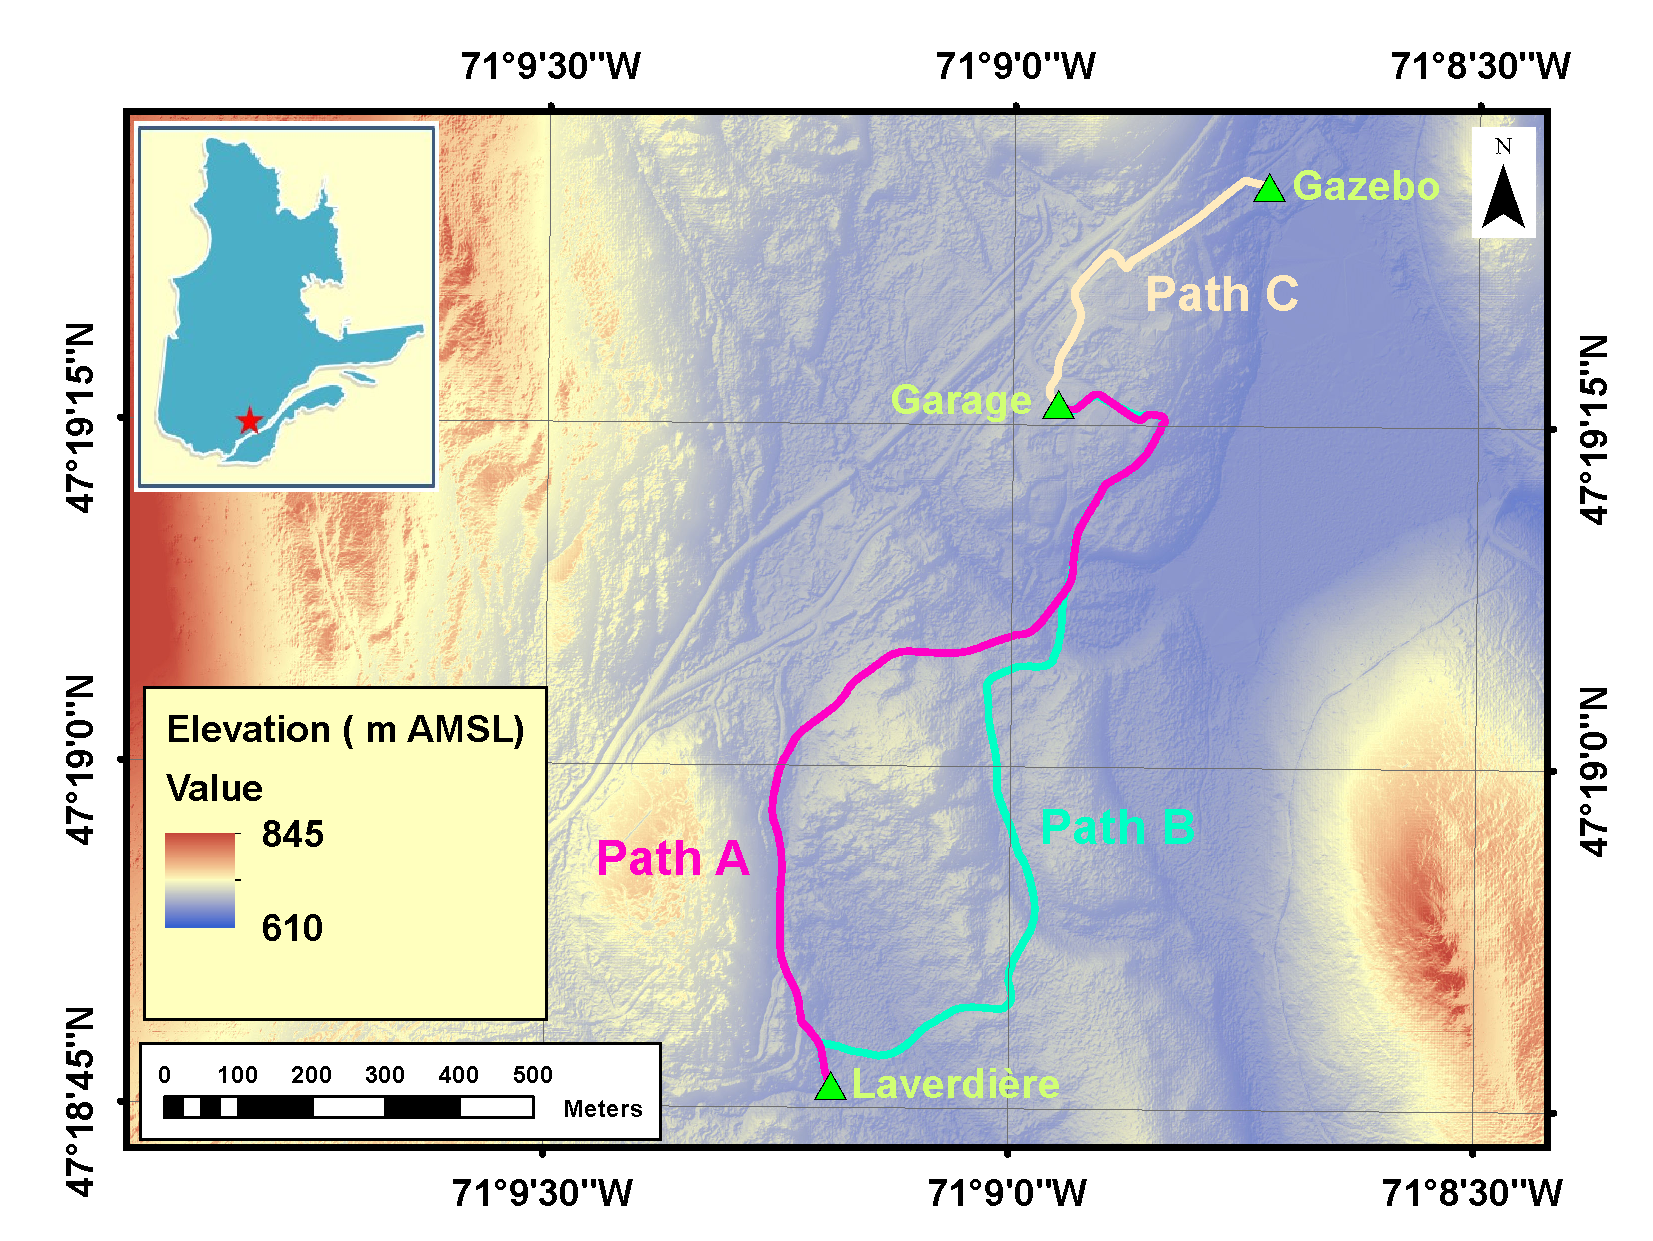
\includegraphics[width=\linewidth]{figs/map-dem.pdf}
			%\caption{A view from above the \textit{Montmorency} forest, which covers \SI{400}{km^2}.}
			\label{fig:view_above}
		\end{subfigure}%
		~~
		\begin{subfigure}[b]{0.45\textwidth}
			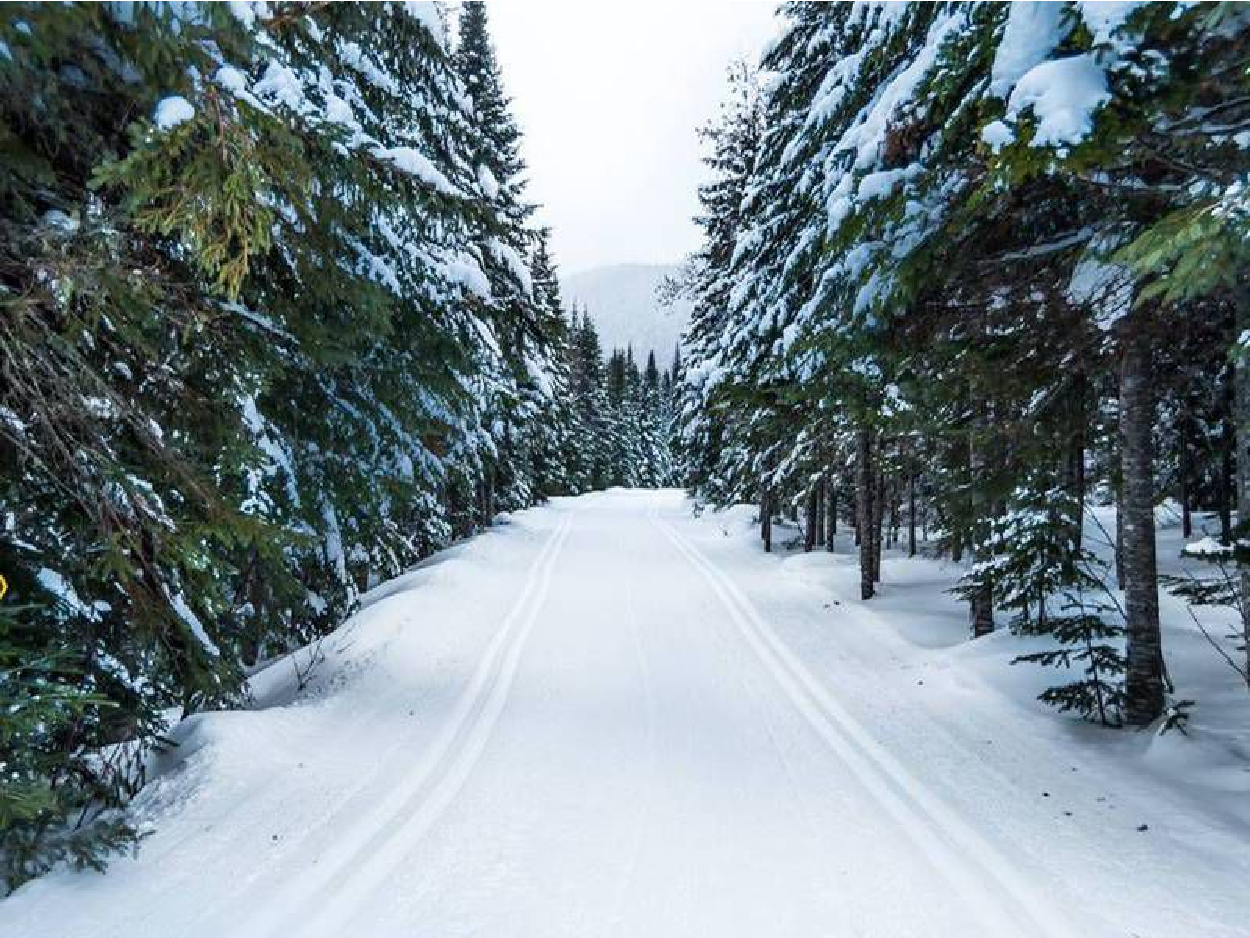
\includegraphics[width=\linewidth]{figs/foret-montmorency-path.pdf}
			%\caption{An example of a snowy path, in which our system performed \ac{LTR}.}
			\label{fig:view_path}
		\end{subfigure}%
		%% Maybe change with a camera image?
		\caption{A digital terrain model of the area where our \ac{LTR} system was deployed.
		We see the three different paths, both the A (\SI{1.5}{km}) and B path ({1.5}{km}) going from the garage \ac{POI} to the \laverdiere~\ac{POI}, while the C path (\SI{0.6}{km}) goes to the Gazebo \ac{POI}.
		The image on the right is an example of the A and B paths, which mostly consists of cross-country sky trails.
		Image credit : \foretmo.} 
		\label{fig:forest}
	\end{center}
\end{figure}

During the five days deployment, we completed
% Discuss weather

\begin{figure} [htpb]
	\centering
	\includegraphics[height=2.0in]{example-image}
	\caption{Johann's various runs and meteo figure}
	\label{fig:meteo_runs}
\end{figure}

\begin{table}[htpb]
	\caption{Overview of all runs realized in this work. 
		All times are defined in the local Eastern Standard Time. 
		The column $\Delta t$ defines the elapsed time since the teach run of the associated path.} \label{tab:all_runs}
	\begin{center}
		\begin{tabular}{c c c c c c}
			\hline
			% after \\: \hline or \cline{col1-col2} \cline{col3-col4} ...
			ID & Path & Start time & Duration & $\Delta t$ & Number of scans \\
			\hline
			TeachA & A & \DTMdate{2021-03-30} \DTMtime{11:04:00} & \DTMtime{00:25:00} & Teach Pass &  \\
			TeachB & B' & \DTMdate{2021-03-29} \DTMtime{15:45:00} & \DTMtime{00:31:00} & Teach Pass \\
			TeachC & C & \DTMdate{2021-03-30} \DTMtime{07:28:00} & \DTMtime{00:15:00} & Teach Pass \\
			R1 & C & \DTMdate{2021-03-31} \DTMtime{10:42:00} & \DTMtime{00:22:00} & \DTMtime{27:14:00} & 17273  \\
			R2 & B & \DTMdate{2021-03-31} \DTMtime{14:03:00} & \DTMtime{00:26:00} & \DTMtime{30:35:00} & 22106  \\
			R3 & A' & \DTMdate{2021-03-31} \DTMtime{15:02:00} & \DTMtime{00:27:00} & \DTMtime{31:34:00} & 16851  \\
			R4 & A & \DTMdate{2021-03-31} \DTMtime{20:42:00} & \DTMtime{00:26:00} & \DTMtime{37:14:00} & 16740  \\
			R5 & B' & \DTMdate{2021-03-31} \DTMtime{21:12:00} & \DTMtime{00:33:00} & \DTMtime{37:44:00} & 18476 \\
			R6 & B & \DTMdate{2021-03-31} \DTMtime{22:00:00} & \DTMtime{00:35:00} & \DTMtime{38:32:00} & 19296 \\
			R7 & A' & \DTMdate{2021-03-31} \DTMtime{22:47:00} & Battery breakdown & \DTMtime{39:19:00} & 10601  \\
			R8 & A & \DTMdate{2021-04-01} \DTMtime{09:21:00} & \DTMtime{00:16:00} & \DTMtime{49:53:00} & 18442  \\
			R9 & B' & \DTMdate{2021-04-01} \DTMtime{10:19:00} & \DTMtime{00:29:00} & \DTMtime{50:51:00} & 20941 \\
			R10 & C & \DTMdate{2021-04-01} \DTMtime{11:01:00} & \DTMtime{00:23:00} & \DTMtime{51:33:00} & 14208 \\
			R11 & B & \DTMdate{2021-04-01} \DTMtime{18:13:00} & \DTMtime{00:23:00} & \DTMtime{58:45:00} & 23214 \\
			R12 & A' & \DTMdate{2021-04-01} \DTMtime{19:09:00} & \DTMtime{00:00:00} & \DTMtime{59:41:00} & 23602 \\
			R13 & A & \DTMdate{2021-04-02} \DTMtime{06:53:00} & \DTMtime{00:26:00} & \DTMtime{71:25:00} & 16840 \\
			R14 & B' & \DTMdate{2021-04-02} \DTMtime{07:25:00} & \DTMtime{00:29:00} & \DTMtime{71:57:00} & 18049 \\
			
		\end{tabular}
	\end{center}
\end{table}

% Check the labels

\begin{figure}[htpb]
	\begin{center}
		\begin{subfigure}[b]{0.32\textwidth}
			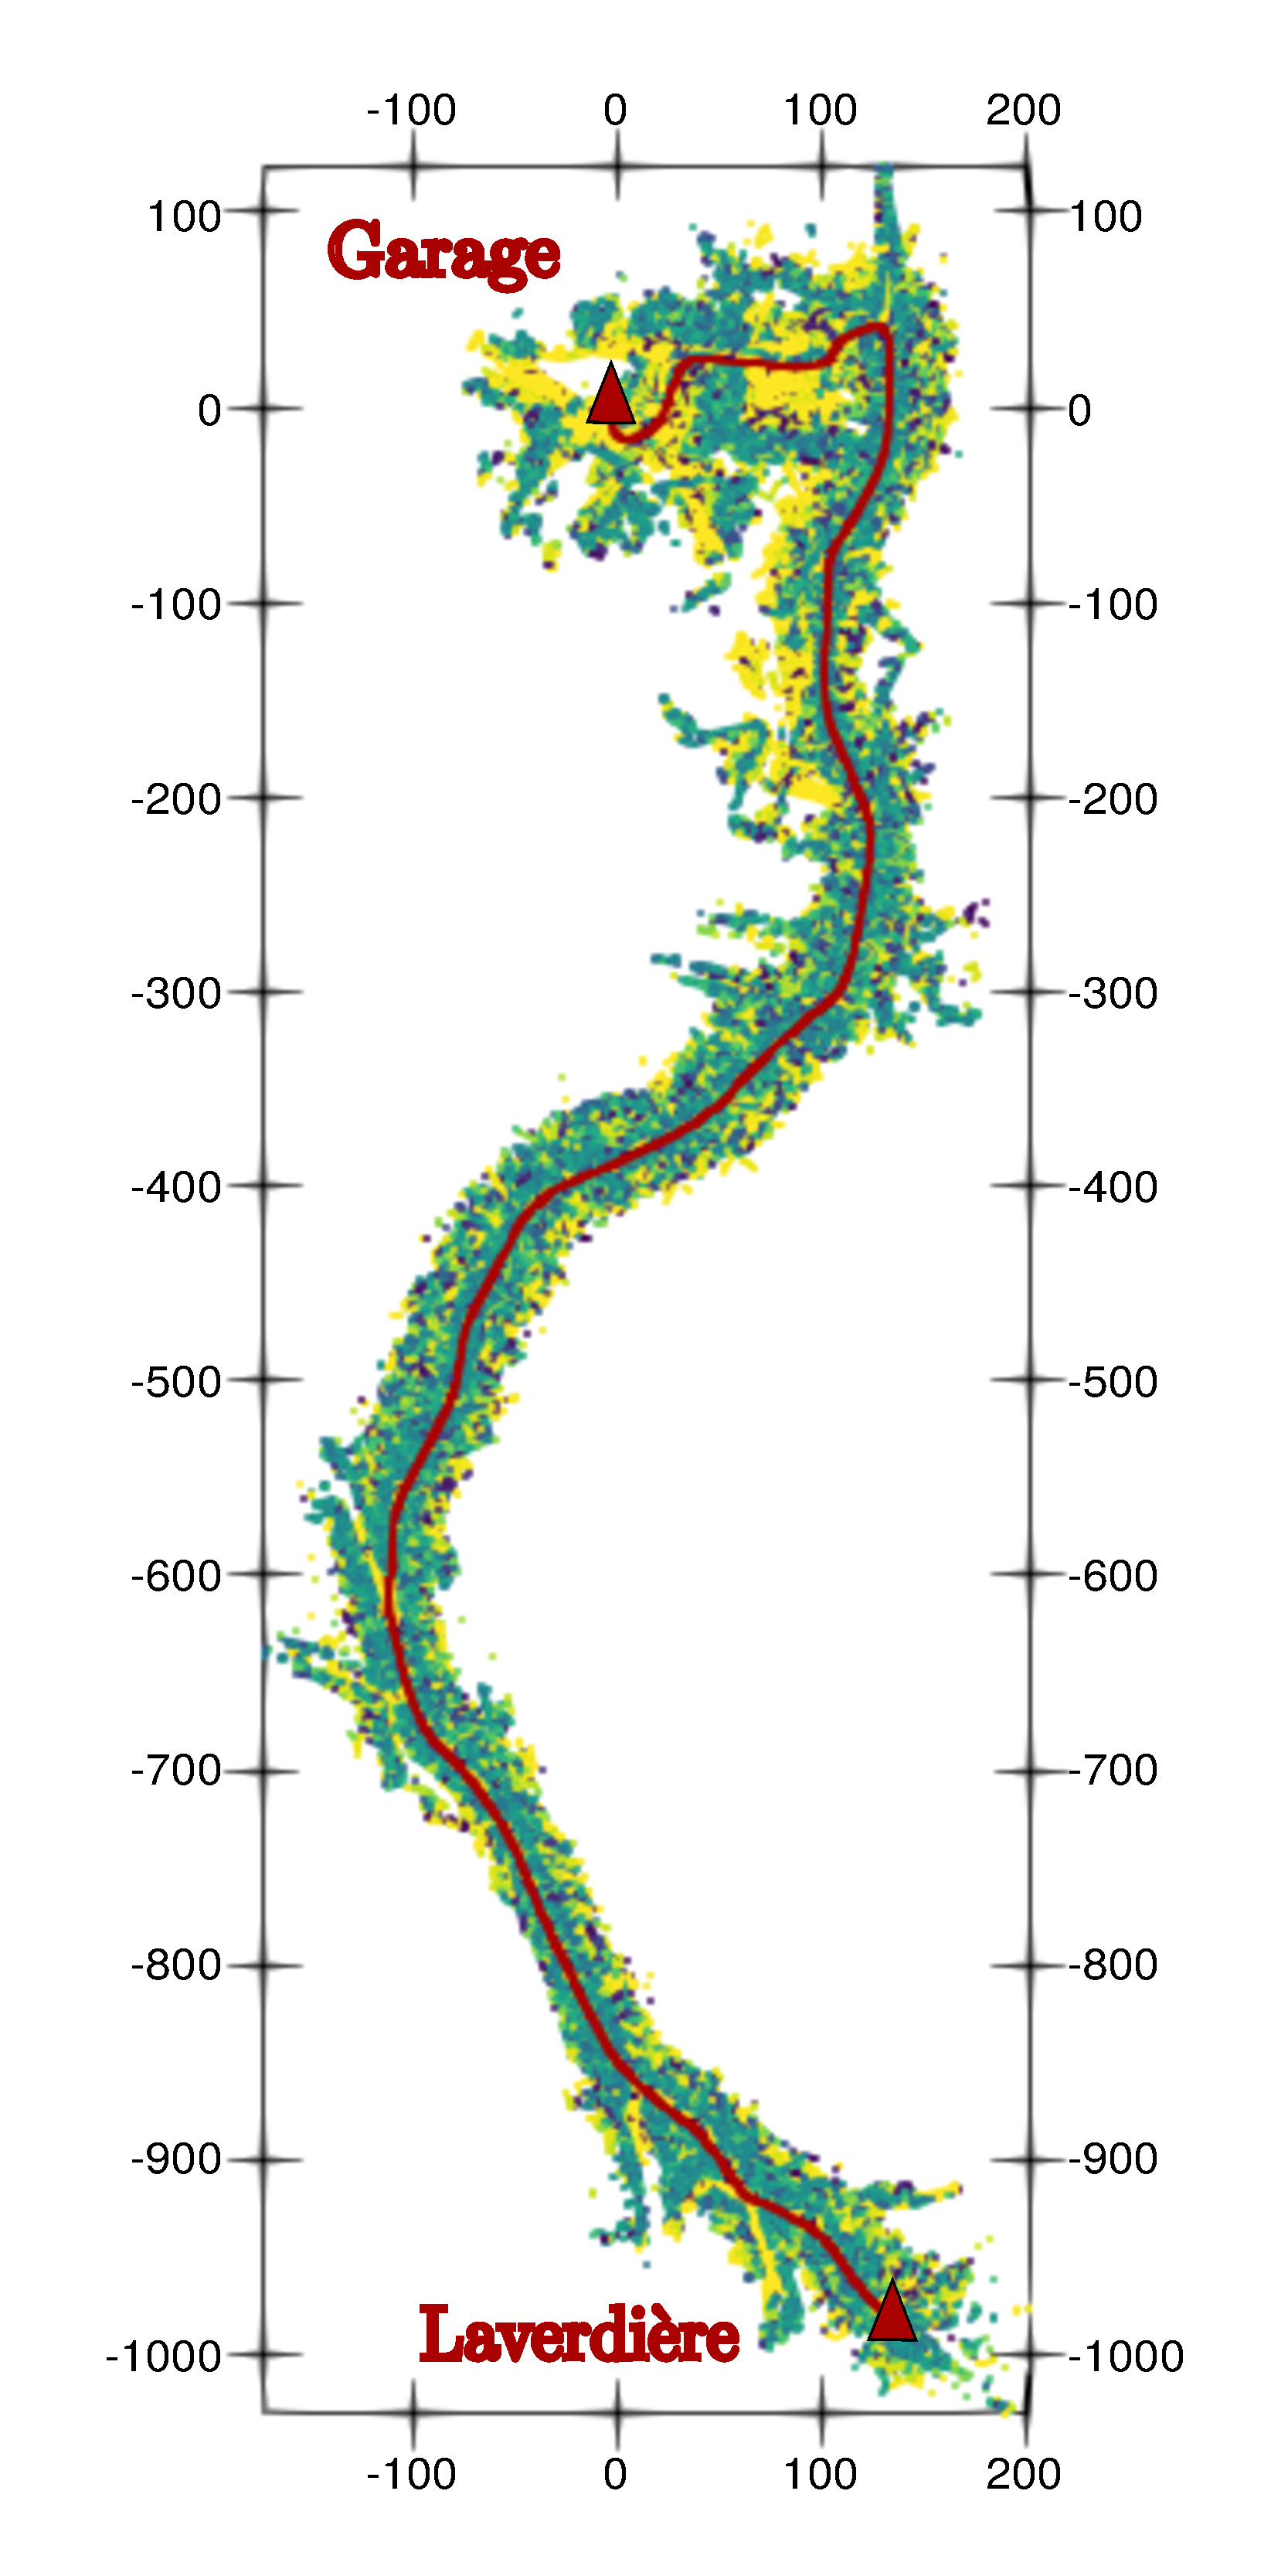
\includegraphics[width=\linewidth]{figs/ltr_map_traj/path_a.pdf}
			%\caption{A view from above the \textit{Montmorency} forest, which covers \SI{400}{km^2}.}
			\label{fig:ltr_a}
			\caption{Path A}
		\end{subfigure}%
		~
		\begin{subfigure}[b]{0.32\textwidth}
			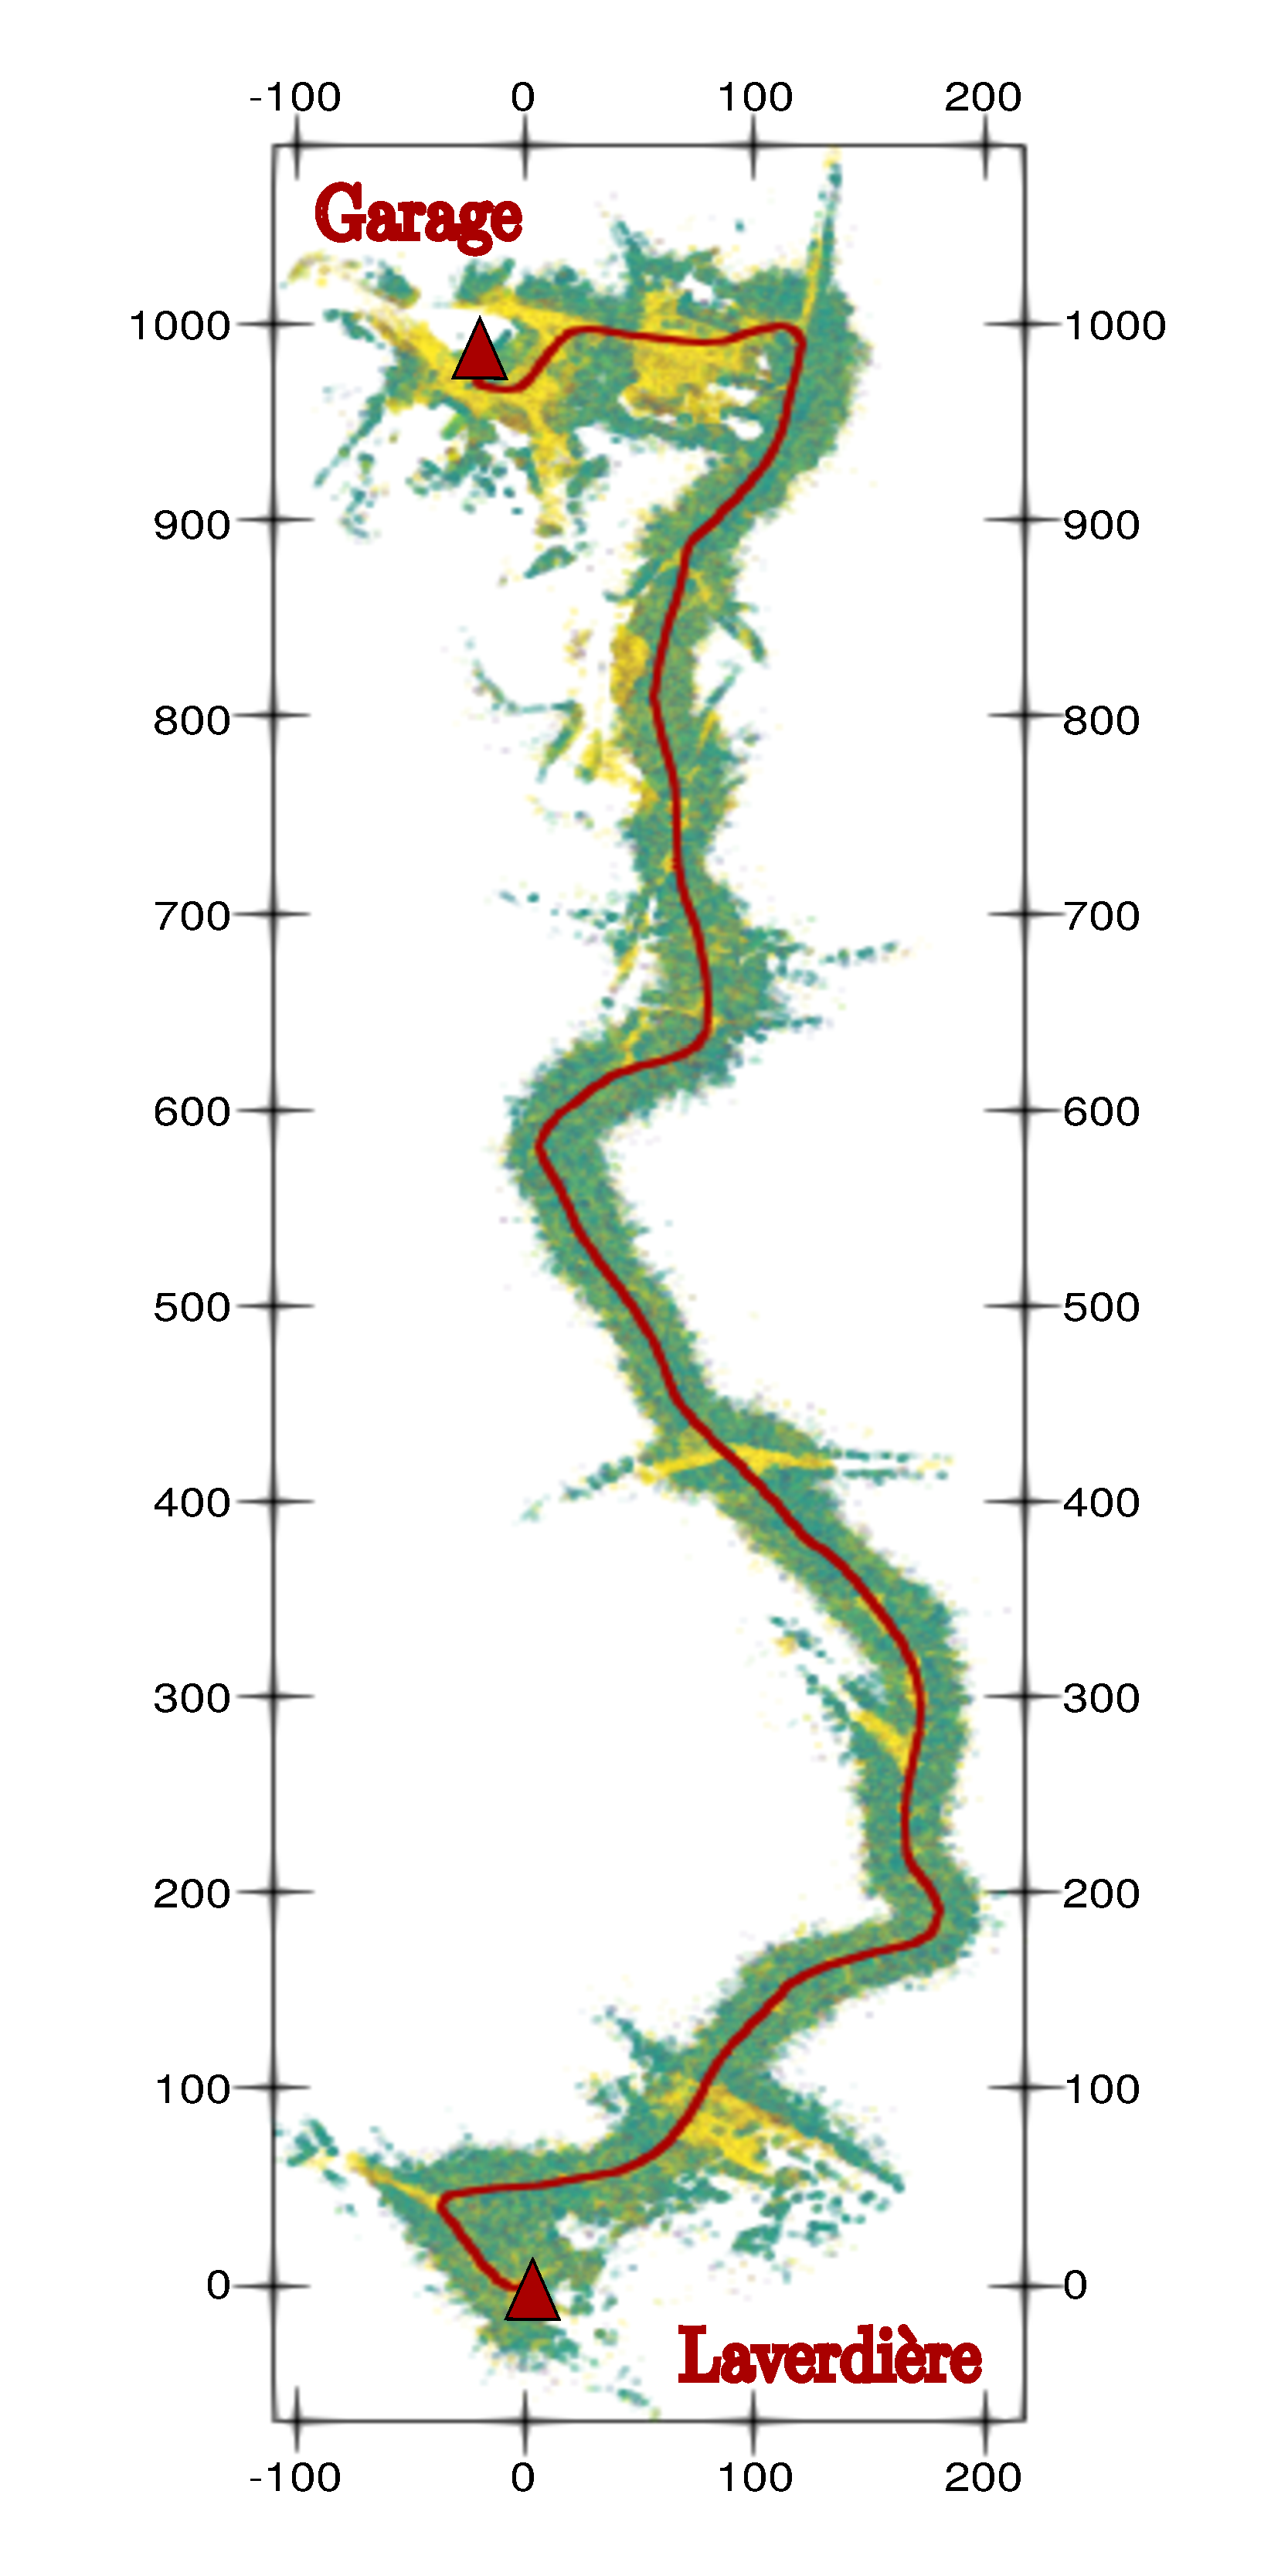
\includegraphics[width=\linewidth]{figs/ltr_map_traj/path_b.pdf}
			%\caption{An example of a snowy path, in which our system performed \ac{LTR}.}
			\label{fig:ltr_b}
			\caption{Path B}
		\end{subfigure}%
		~
		\begin{subfigure}[b]{0.32\textwidth}
			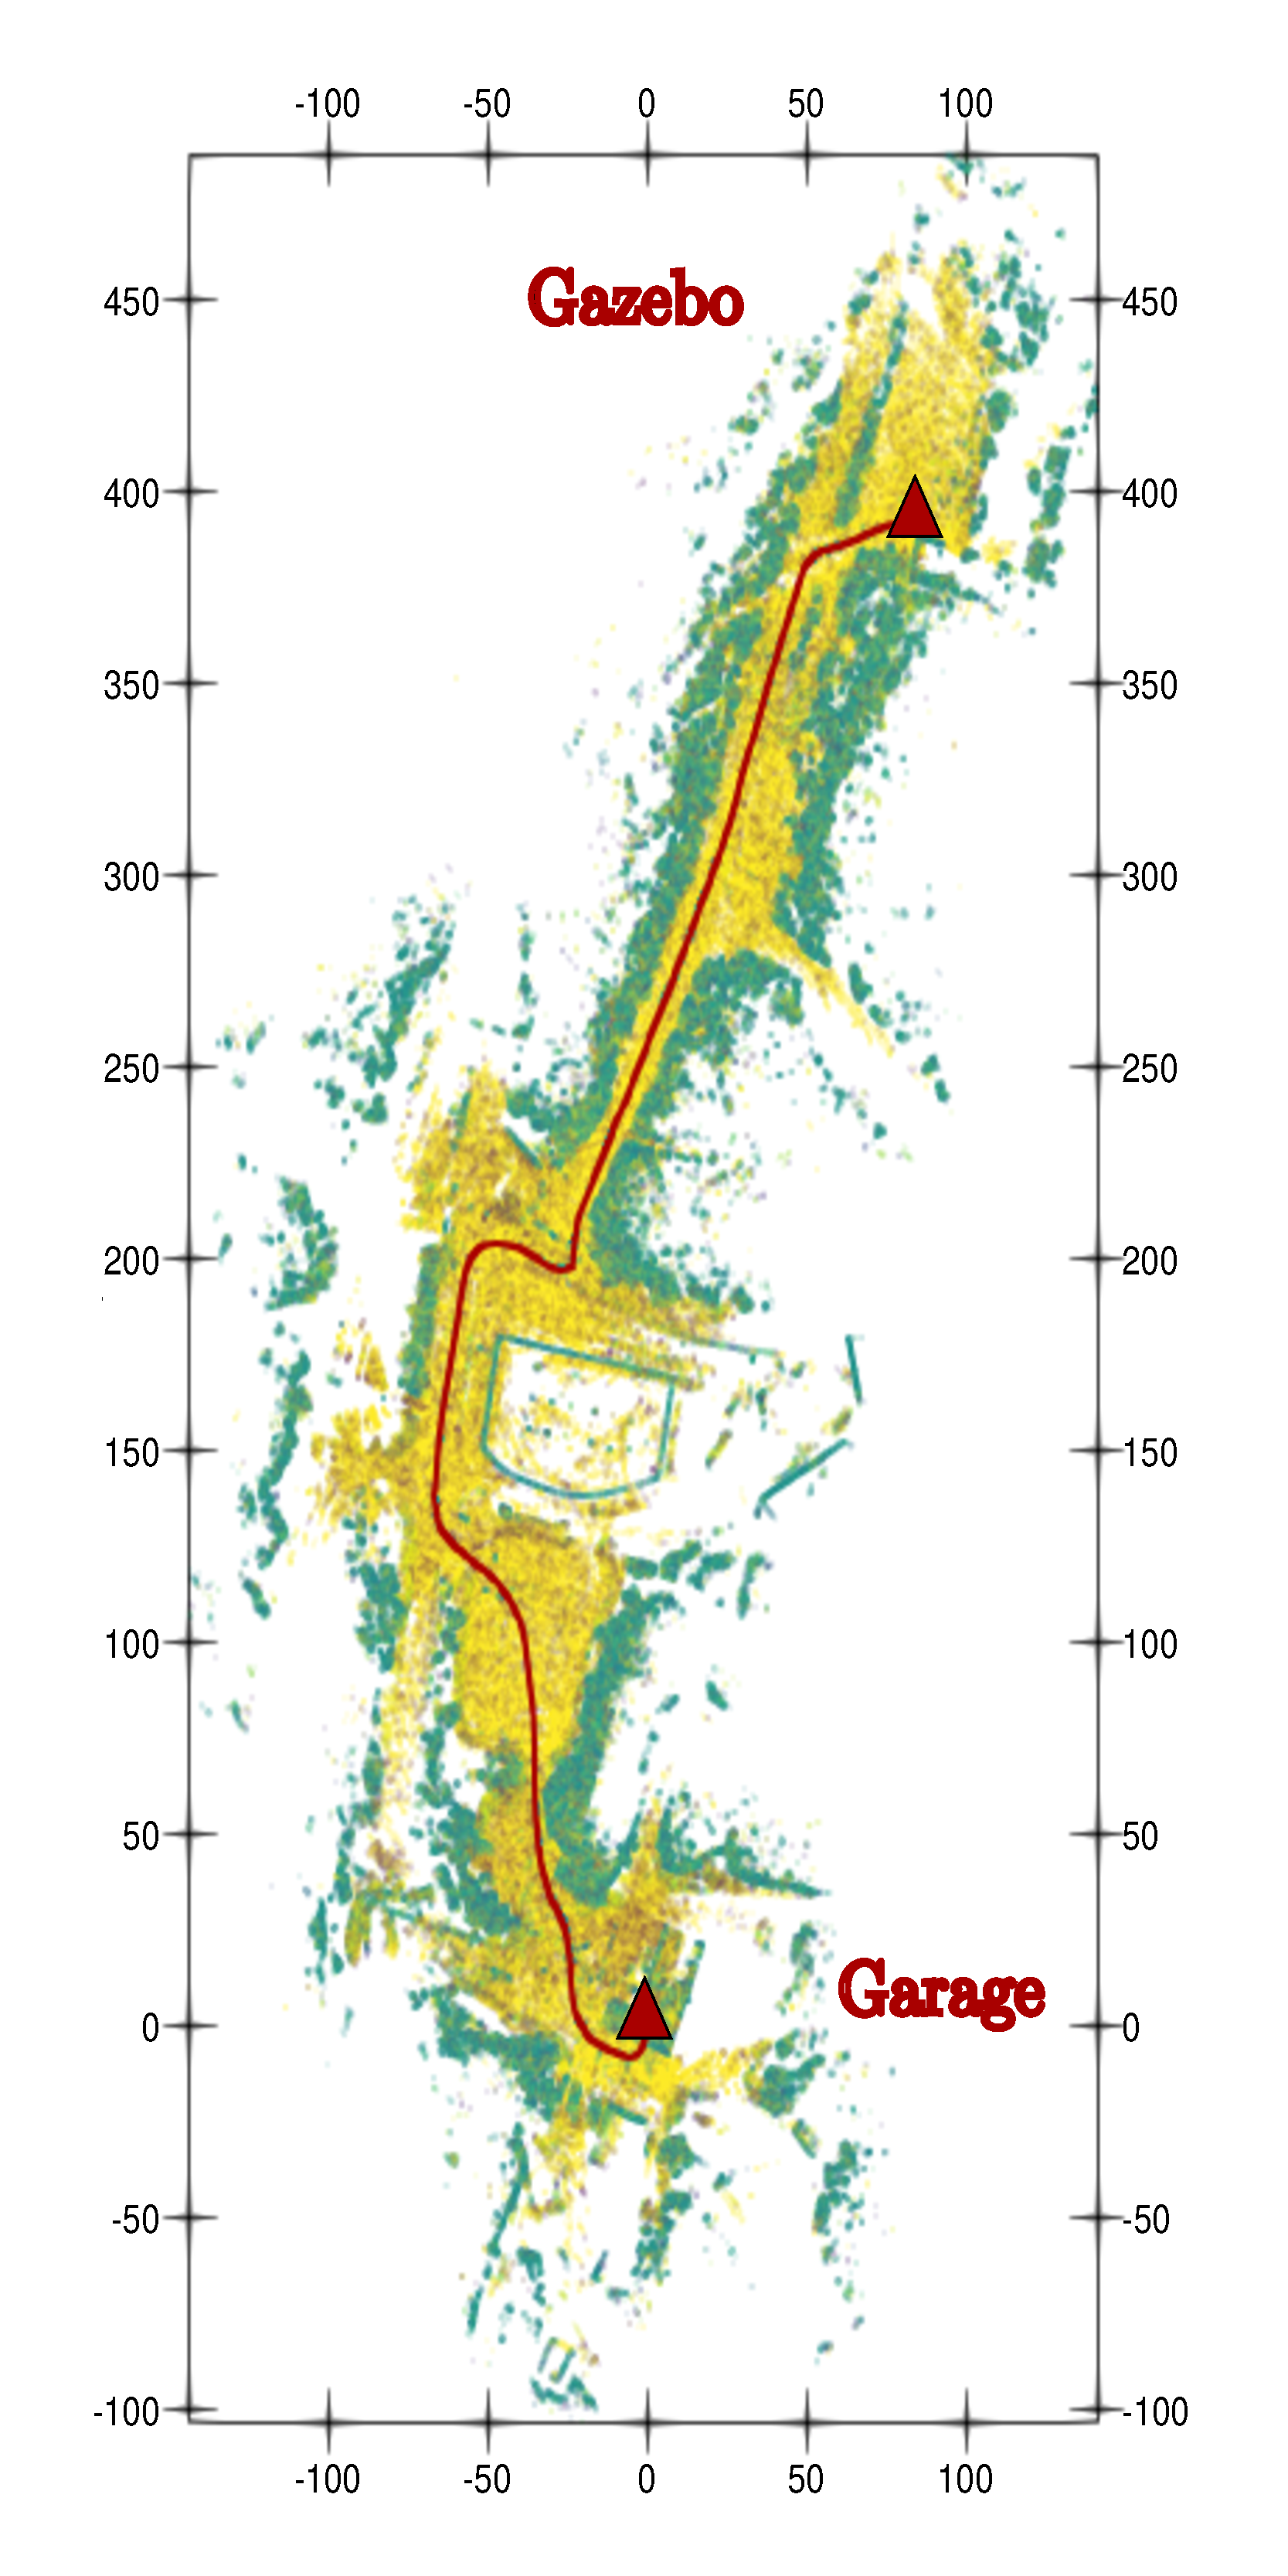
\includegraphics[width=\linewidth]{figs/ltr_map_traj/path_c.pdf}
			%\caption{An example of a snowy path, in which our system performed \ac{LTR}.}
			\label{fig:ltr_c}
			\caption{Path C}
		\end{subfigure}%
		%% Maybe change with a camera image?
		\caption{All reference trajectories and maps recorder for this work.
		In yellow are points with the surface normals pointing upwards, typically representing the ground.
		In green are points with surface normals pointing sideways, typically representing walls or trees.
		In red is the reference trajectory and their respective \acp{POI}.} 
		\label{fig:forest}
	\end{center}
\end{figure}

% Validate run durations through bag files

% Number of points per maps : 
%Map A: 1729505 points
%Map B: 2423769 points
%Map C: 637690 points

\lightlipsum[1]